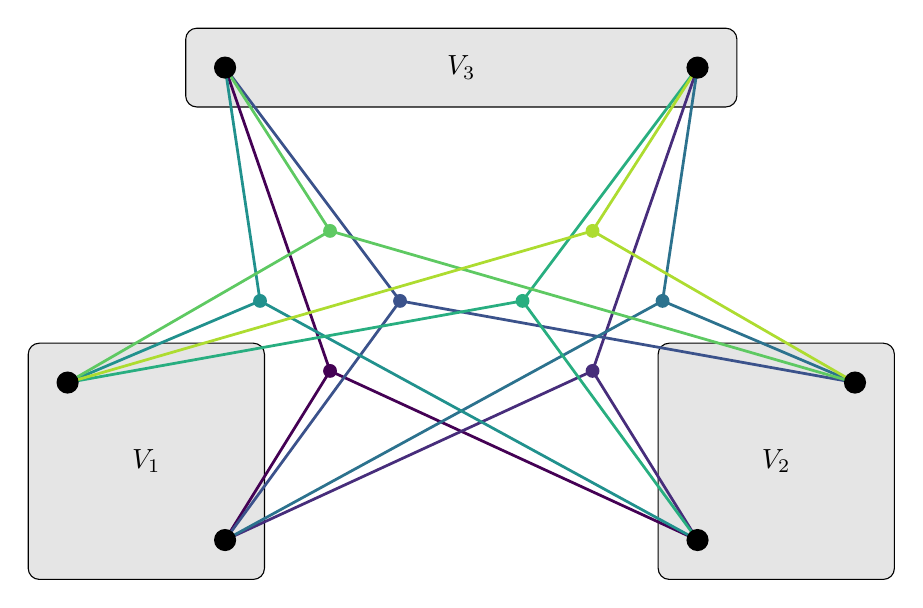
\begin{tikzpicture}[scale=1]
\draw[fill=gray!20, rounded corners] (-0.5, -0.5) rectangle (2.5, 2.5);
\node at (1.0, 1.0) [align=center] {$V_1$};
\draw[fill=gray!20, rounded corners] (7.5, -0.5) rectangle (10.5, 2.5);
\node at (9.0, 1.0) [align=center] {$V_2$};
\draw[fill=gray!20, rounded corners] (1.5, 5.5) rectangle (8.5, 6.5);
\node at (5.0, 6.0) [align=center] {$V_3$};
\coordinate (A1) at (2, 0);
\coordinate (A2) at (0, 2);
\coordinate (B1) at (8, 0);
\coordinate (B2) at (10, 2);
\coordinate (C1) at (2, 6);
\coordinate (C2) at (8, 6);
\definecolor{edgecolor0}{rgb}{0.267, 0.005, 0.329}
\coordinate (R0) at (3.333, 2.148);
\draw[line width=1.0pt, color=edgecolor0] (R0) -- (A1);
\draw[line width=1.0pt, color=edgecolor0] (R0) -- (B1);
\draw[line width=1.0pt, color=edgecolor0] (R0) -- (C1);
\fill[color=edgecolor0] (R0) circle (2.5pt);
\definecolor{edgecolor1}{rgb}{0.279, 0.175, 0.483}
\coordinate (R1) at (6.667, 2.148);
\draw[line width=1.0pt, color=edgecolor1] (R1) -- (A1);
\draw[line width=1.0pt, color=edgecolor1] (R1) -- (B1);
\draw[line width=1.0pt, color=edgecolor1] (R1) -- (C2);
\fill[color=edgecolor1] (R1) circle (2.5pt);
\definecolor{edgecolor2}{rgb}{0.230, 0.322, 0.546}
\coordinate (R2) at (4.222, 3.037);
\draw[line width=1.0pt, color=edgecolor2] (R2) -- (A1);
\draw[line width=1.0pt, color=edgecolor2] (R2) -- (B2);
\draw[line width=1.0pt, color=edgecolor2] (R2) -- (C1);
\fill[color=edgecolor2] (R2) circle (2.5pt);
\definecolor{edgecolor3}{rgb}{0.173, 0.449, 0.558}
\coordinate (R3) at (7.556, 3.037);
\draw[line width=1.0pt, color=edgecolor3] (R3) -- (A1);
\draw[line width=1.0pt, color=edgecolor3] (R3) -- (B2);
\draw[line width=1.0pt, color=edgecolor3] (R3) -- (C2);
\fill[color=edgecolor3] (R3) circle (2.5pt);
\definecolor{edgecolor4}{rgb}{0.128, 0.567, 0.551}
\coordinate (R4) at (2.444, 3.037);
\draw[line width=1.0pt, color=edgecolor4] (R4) -- (A2);
\draw[line width=1.0pt, color=edgecolor4] (R4) -- (B1);
\draw[line width=1.0pt, color=edgecolor4] (R4) -- (C1);
\fill[color=edgecolor4] (R4) circle (2.5pt);
\definecolor{edgecolor5}{rgb}{0.158, 0.684, 0.502}
\coordinate (R5) at (5.778, 3.037);
\draw[line width=1.0pt, color=edgecolor5] (R5) -- (A2);
\draw[line width=1.0pt, color=edgecolor5] (R5) -- (B1);
\draw[line width=1.0pt, color=edgecolor5] (R5) -- (C2);
\fill[color=edgecolor5] (R5) circle (2.5pt);
\definecolor{edgecolor6}{rgb}{0.369, 0.789, 0.383}
\coordinate (R6) at (3.333, 3.926);
\draw[line width=1.0pt, color=edgecolor6] (R6) -- (A2);
\draw[line width=1.0pt, color=edgecolor6] (R6) -- (B2);
\draw[line width=1.0pt, color=edgecolor6] (R6) -- (C1);
\fill[color=edgecolor6] (R6) circle (2.5pt);
\definecolor{edgecolor7}{rgb}{0.678, 0.864, 0.190}
\coordinate (R7) at (6.667, 3.926);
\draw[line width=1.0pt, color=edgecolor7] (R7) -- (A2);
\draw[line width=1.0pt, color=edgecolor7] (R7) -- (B2);
\draw[line width=1.0pt, color=edgecolor7] (R7) -- (C2);
\fill[color=edgecolor7] (R7) circle (2.5pt);
\fill[black] (A1) circle (4.0pt);
\fill[black] (A2) circle (4.0pt);
\fill[black] (B1) circle (4.0pt);
\fill[black] (B2) circle (4.0pt);
\fill[black] (C1) circle (4.0pt);
\fill[black] (C2) circle (4.0pt);
\end{tikzpicture}